\documentclass{article}
\usepackage[utf8]{inputenc}
\usepackage[top=1in]{geometry}
\usepackage{graphicx}
\usepackage{booktabs}
\usepackage{amsmath}
\usepackage{amsthm}
\usepackage[only]{excludeonly}
\usepackage{fancyhdr}
\usepackage{tikz}
\usetikzlibrary{circuits.logic.US,positioning,calc} 
\usepackage[american]{circuitikz}

\usepackage{enumitem,amssymb}
\newlist{todolist}{itemize}{2}
\setlist[todolist]{label=$\square$}
\usepackage{pifont}
\newcommand{\cmark}{\ding{51}}%
\newcommand{\xmark}{\ding{55}}%
\newcommand{\done}{\rlap{$\square$}{\raisebox{2pt}{\large\hspace{1pt}\cmark}}%
  \hspace{-2.5pt}}
\newcommand{\wontfix}{\rlap{$\square$}{\large\hspace{1pt}\xmark}}

% https://tex.stackexchange.com/questions/140567/drawing-karnaughs-maps-in-latex
\usepackage{tikz}
\usetikzlibrary{matrix,calc}

%isolated term
%#1 - Optional. Space between node and grouping line. Default=0
%#2 - node
%#3 - filling color
\newcommand{\implicantsol}[3][0]{
    \draw[rounded corners=3pt, fill=#3, opacity=0.3] ($(#2.north west)+(135:#1)$) rectangle ($(#2.south east)+(-45:#1)$);
    }


%internal group
%#1 - Optional. Space between node and grouping line. Default=0
%#2 - top left node
%#3 - bottom right node
%#4 - filling color
\newcommand{\implicant}[4][0]{
    \draw[rounded corners=3pt, fill=#4, opacity=0.3] ($(#2.north west)+(135:#1)$) rectangle ($(#3.south east)+(-45:#1)$);
    }

%group lateral borders
%#1 - Optional. Space between node and grouping line. Default=0
%#2 - top left node
%#3 - bottom right node
%#4 - filling color
\newcommand{\implicantcostats}[4][0]{
    \draw[rounded corners=3pt, fill=#4, opacity=0.3] ($(rf.east |- #2.north)+(90:#1)$)-| ($(#2.east)+(0:#1)$) |- ($(rf.east |- #3.south)+(-90:#1)$);
    \draw[rounded corners=3pt, fill=#4, opacity=0.3] ($(cf.west |- #2.north)+(90:#1)$) -| ($(#3.west)+(180:#1)$) |- ($(cf.west |- #3.south)+(-90:#1)$);
}

%group top-bottom borders
%#1 - Optional. Space between node and grouping line. Default=0
%#2 - top left node
%#3 - bottom right node
%#4 - filling color
\newcommand{\implicantdaltbaix}[4][0]{
    \draw[rounded corners=3pt, fill=#4, opacity=0.3] ($(cf.south -| #2.west)+(180:#1)$) |- ($(#2.south)+(-90:#1)$) -| ($(cf.south -| #3.east)+(0:#1)$);
    \draw[rounded corners=3pt, fill=#4, opacity=0.3] ($(rf.north -| #2.west)+(180:#1)$) |- ($(#3.north)+(90:#1)$) -| ($(rf.north -| #3.east)+(0:#1)$);
}

%group corners
%#1 - Optional. Space between node and grouping line. Default=0
%#2 - filling color
\newcommand{\implicantcantons}[2][0]{
    \draw[rounded corners=3pt, opacity=.3] ($(rf.east |- 0.south)+(-90:#1)$) -| ($(0.east |- cf.south)+(0:#1)$);
    \draw[rounded corners=3pt, opacity=.3] ($(rf.east |- 8.north)+(90:#1)$) -| ($(8.east |- rf.north)+(0:#1)$);
    \draw[rounded corners=3pt, opacity=.3] ($(cf.west |- 2.south)+(-90:#1)$) -| ($(2.west |- cf.south)+(180:#1)$);
    \draw[rounded corners=3pt, opacity=.3] ($(cf.west |- 10.north)+(90:#1)$) -| ($(10.west |- rf.north)+(180:#1)$);
    \fill[rounded corners=3pt, fill=#2, opacity=.3] ($(rf.east |- 0.south)+(-90:#1)$) -|  ($(0.east |- cf.south)+(0:#1)$) [sharp corners] ($(rf.east |- 0.south)+(-90:#1)$) |-  ($(0.east |- cf.south)+(0:#1)$) ;
    \fill[rounded corners=3pt, fill=#2, opacity=.3] ($(rf.east |- 8.north)+(90:#1)$) -| ($(8.east |- rf.north)+(0:#1)$) [sharp corners] ($(rf.east |- 8.north)+(90:#1)$) |- ($(8.east |- rf.north)+(0:#1)$) ;
    \fill[rounded corners=3pt, fill=#2, opacity=.3] ($(cf.west |- 2.south)+(-90:#1)$) -| ($(2.west |- cf.south)+(180:#1)$) [sharp corners]($(cf.west |- 2.south)+(-90:#1)$) |- ($(2.west |- cf.south)+(180:#1)$) ;
    \fill[rounded corners=3pt, fill=#2, opacity=.3] ($(cf.west |- 10.north)+(90:#1)$) -| ($(10.west |- rf.north)+(180:#1)$) [sharp corners] ($(cf.west |- 10.north)+(90:#1)$) |- ($(10.west |- rf.north)+(180:#1)$) ;
}

%Empty Karnaugh map 4x4
\newenvironment{Karnaugh}[2]%
{
\begin{tikzpicture}[baseline=(current bounding box.north),scale=0.8]
\draw (0,0) grid (4,4);
\draw (0,4) -- node [pos=0.7,above right,anchor=south west] {#1} node [pos=0.7,below left,anchor=north east] {#2} ++(135:1);
%
\matrix (mapa) [matrix of nodes,
        column sep={0.8cm,between origins},
        row sep={0.8cm,between origins},
        every node/.style={minimum size=0.3mm},
        anchor=2.center,
        ampersand replacement=\&] at (0.5,0.5)
{
                       \& |(c00)| 00         \& |(c01)| 01         \& |(c11)| 11         \& |(c10)| 10         \& |(cf)| \phantom{00} \\
|(r00)| 00             \& |(0)|  \phantom{0} \& |(4)|  \phantom{0} \& |(12)|  \phantom{0} \& |(8)|  \phantom{0} \&                     \\
|(r01)| 01             \& |(1)|  \phantom{0} \& |(5)|  \phantom{0} \& |(13)|  \phantom{0} \& |(9)|  \phantom{0} \&                     \\
|(r11)| 11             \& |(3)| \phantom{0} \& |(7)| \phantom{0} \& |(15)| \phantom{0} \& |(11)| \phantom{0} \&                     \\
|(r10)| 10             \& |(2)|  \phantom{0} \& |(6)|  \phantom{0} \& |(14)| \phantom{0} \& |(10)| \phantom{0} \&                     \\
|(rf) | \phantom{00}   \&                    \&                    \&                    \&                    \&                     \\
};
}%
{
\end{tikzpicture}
}

%Empty Karnaugh map 2x4
\newenvironment{Karnaughvuit}%
{
\begin{tikzpicture}[baseline=(current bounding box.north),scale=0.8]
\draw (0,0) grid (4,2);
\draw (0,2) -- node [pos=0.7,above right,anchor=south west] {AB} node [pos=0.7,below left,anchor=north east] {C} ++(135:1);
%
\matrix (mapa) [matrix of nodes,
        column sep={0.8cm,between origins},
        row sep={0.8cm,between origins},
        every node/.style={minimum size=0.3mm},
        anchor=1.center,
        ampersand replacement=\&] at (0.5,0.5)
{
                      \& |(c00)| 00         \& |(c01)| 01         \& |(c11)| 11         \& |(c10)| 10         \& |(cf)| \phantom{00} \\
|(r00)| 0             \& |(0)|  \phantom{0} \& |(2)|  \phantom{0} \& |(6)|  \phantom{0} \& |(4)|  \phantom{0} \&                     \\
|(r01)| 1             \& |(1)|  \phantom{0} \& |(3)|  \phantom{0} \& |(7)|  \phantom{0} \& |(5)|  \phantom{0} \&                     \\
|(rf) | \phantom{00}  \&                    \&                    \&                    \&                    \&                     \\
};
}%
{
\end{tikzpicture}
}

%Empty Karnaugh map 2x2
\newenvironment{Karnaughquatre}%
{
\begin{tikzpicture}[baseline=(current bounding box.north),scale=0.8]
\draw (0,0) grid (2,2);
\draw (0,2) -- node [pos=0.7,above right,anchor=south west] {A} node [pos=0.7,below left,anchor=north east] {B} ++(135:1);
%
\matrix (mapa) [matrix of nodes,
        column sep={0.8cm,between origins},
        row sep={0.8cm,between origins},
        every node/.style={minimum size=0.3mm},
        anchor=1.center,
        ampersand replacement=\&] at (0.5,0.5)
{
          \& |(c00)| 0          \& |(c01)| 1  \\
|(r00)| 0 \& |(0)|  \phantom{0} \& |(2)|  \phantom{0} \\
|(r01)| 1 \& |(1)|  \phantom{0} \& |(3)|  \phantom{0} \\
};
}%
{
\end{tikzpicture}
}

%Defines 8 or 16 values (0,1,X)
\newcommand{\contingut}[1]{%
\foreach \x [count=\xi from 0]  in {#1}
     \path (\xi) node {\x};
}

%Places 1 in listed positions
\newcommand{\minterms}[1]{%
    \foreach \x in {#1}
        \path (\x) node {1};
}

%Places 0 in listed positions
\newcommand{\maxterms}[1]{%
    \foreach \x in {#1}
        \path (\x) node {0};
}

%Places X in listed positions
\newcommand{\indeterminats}[1]{%
    \foreach \x in {#1}
        \path (\x) node {X};
}

% Places m_{x} in listed positions
\newcommand{\phminterms}[1]{%
  \foreach \x in {#1}
  \path (\x) node {$m_{\x}$};
}

% Places m_{16+x} in listed positions
\newcommand{\phmintermssixt}[1]{%
  \foreach [evaluate={\y=int(16+\x)}] \x in {#1}
  \path (\x) node {$m_{\y}$};
}

% Calligraphic fonts
\newcommand{\calA}{{\cal A}}
\newcommand{\calB}{{\cal B}}
\newcommand{\calC}{{\cal C}}
\newcommand{\calD}{{\cal D}}
\newcommand{\calE}{{\cal E}}
\newcommand{\calF}{{\cal F}}
\newcommand{\calG}{{\cal G}}
\newcommand{\calH}{{\cal H}}
\newcommand{\calI}{{\cal I}}
\newcommand{\calJ}{{\cal J}}
\newcommand{\calK}{{\cal K}}
\newcommand{\calL}{{\cal L}}
\newcommand{\calM}{{\cal M}}
\newcommand{\calN}{{\cal N}}
\newcommand{\calO}{{\cal O}}
\newcommand{\calP}{{\cal P}}
\newcommand{\calQ}{{\cal Q}}
\newcommand{\calR}{{\cal R}}
\newcommand{\calS}{{\cal S}}
\newcommand{\calT}{{\cal T}}
\newcommand{\calU}{{\cal U}}
\newcommand{\calV}{{\cal V}}
\newcommand{\calW}{{\cal W}}
\newcommand{\calX}{{\cal X}}
\newcommand{\calY}{{\cal Y}}
\newcommand{\calZ}{{\cal Z}}

% Sets:
\newcommand{\setA}{\textsf{A}}
\newcommand{\setB}{\textsf{B}}
\newcommand{\setC}{\textsf{C}}
\newcommand{\setD}{\textsf{D}}
\newcommand{\setE}{\textsf{E}}
\newcommand{\setF}{\textsf{F}}
\newcommand{\setG}{\textsf{G}}
\newcommand{\setH}{\textsf{H}}
\newcommand{\setI}{\textsf{I}}
\newcommand{\setJ}{\textsf{J}}
\newcommand{\setK}{\textsf{K}}
\newcommand{\setL}{\textsf{L}}
\newcommand{\setM}{\textsf{M}}
\newcommand{\setN}{\textsf{N}}
\newcommand{\setO}{\textsf{O}}
\newcommand{\setP}{\textsf{P}}
\newcommand{\setQ}{\textsf{Q}}
\newcommand{\setR}{\textsf{R}}
\newcommand{\setS}{\textsf{S}}
\newcommand{\setT}{\textsf{T}}
\newcommand{\setU}{\textsf{U}}
\newcommand{\setV}{\textsf{V}}
\newcommand{\setW}{\textsf{W}}
\newcommand{\setX}{\textsf{X}}
\newcommand{\setY}{\textsf{Y}}
\newcommand{\setZ}{\textsf{Z}}

% Vectors
\newcommand{\bfa}{\mathbf{a}}
\newcommand{\bfb}{\mathbf{b}}
\newcommand{\bfc}{\mathbf{c}}
\newcommand{\bfd}{\mathbf{d}}
\newcommand{\bfe}{\mathbf{e}}
\newcommand{\bff}{\mathbf{f}}
\newcommand{\bfg}{\mathbf{g}}
\newcommand{\bfh}{\mathbf{h}}
\newcommand{\bfi}{\mathbf{i}}
\newcommand{\bfj}{\mathbf{j}}
\newcommand{\bfk}{\mathbf{k}}
\newcommand{\bfl}{\mathbf{l}}
\newcommand{\bfm}{\mathbf{m}}
\newcommand{\bfn}{\mathbf{n}}
\newcommand{\bfo}{\mathbf{o}}
\newcommand{\bfp}{\mathbf{p}}
\newcommand{\bfq}{\mathbf{q}}
\newcommand{\bfr}{\mathbf{r}}
\newcommand{\bfs}{\mathbf{s}}
\newcommand{\bft}{\mathbf{t}}
\newcommand{\bfu}{\mathbf{u}}
\newcommand{\bfv}{\mathbf{v}}
\newcommand{\bfw}{\mathbf{w}}
\newcommand{\bfx}{\mathbf{x}}
\newcommand{\bfy}{\mathbf{y}}
\newcommand{\bfz}{\mathbf{z}}


\newcommand{\bfalpha}{\boldsymbol{\alpha}}
\newcommand{\bfbeta}{\boldsymbol{\beta}}
\newcommand{\bfgamma}{\boldsymbol{\gamma}}
\newcommand{\bfdelta}{\boldsymbol{\delta}}
\newcommand{\bfepsilon}{\boldsymbol{\epsilon}}
\newcommand{\bfzeta}{\boldsymbol{\zeta}}
\newcommand{\bfeta}{\boldsymbol{\eta}}
\newcommand{\bftheta}{\boldsymbol{\theta}}
\newcommand{\bfiota}{\boldsymbol{\iota}}
\newcommand{\bfkappa}{\boldsymbol{\kappa}}
\newcommand{\bflambda}{\boldsymbol{\lambda}}
\newcommand{\bfmu}{\boldsymbol{\mu}}
\newcommand{\bfnu}{\boldsymbol{\nu}}
\newcommand{\bfomicron}{\boldsymbol{\omicron}}
\newcommand{\bfpi}{\boldsymbol{\pi}}
\newcommand{\bfrho}{\boldsymbol{\rho}}
\newcommand{\bfsigma}{\boldsymbol{\sigma}}
\newcommand{\bftau}{\boldsymbol{\tau}}
\newcommand{\bfupsilon}{\boldsymbol{\upsilon}}
\newcommand{\bfphi}{\boldsymbol{\phi}}
\newcommand{\bfchi}{\boldsymbol{\chi}}
\newcommand{\bfpsi}{\boldsymbol{\psi}}
\newcommand{\bfomega}{\boldsymbol{\omega}}
\newcommand{\bfxi}{\boldsymbol{\xi}}
\newcommand{\bfell}{\boldsymbol{\ell}}

% Matrices
\newcommand{\bfA}{\mathbf{A}}
\newcommand{\bfB}{\mathbf{B}}
\newcommand{\bfC}{\mathbf{C}}
\newcommand{\bfD}{\mathbf{D}}
\newcommand{\bfE}{\mathbf{E}}
\newcommand{\bfF}{\mathbf{F}}
\newcommand{\bfG}{\mathbf{G}}
\newcommand{\bfH}{\mathbf{H}}
\newcommand{\bfI}{\mathbf{I}}
\newcommand{\bfJ}{\mathbf{J}}
\newcommand{\bfK}{\mathbf{K}}
\newcommand{\bfL}{\mathbf{L}}
\newcommand{\bfM}{\mathbf{M}}
\newcommand{\bfN}{\mathbf{N}}
\newcommand{\bfO}{\mathbf{O}}
\newcommand{\bfP}{\mathbf{P}}
\newcommand{\bfQ}{\mathbf{Q}}
\newcommand{\bfR}{\mathbf{R}}
\newcommand{\bfS}{\mathbf{S}}
\newcommand{\bfT}{\mathbf{T}}
\newcommand{\bfU}{\mathbf{U}}
\newcommand{\bfV}{\mathbf{V}}
\newcommand{\bfW}{\mathbf{W}}
\newcommand{\bfX}{\mathbf{X}}
\newcommand{\bfY}{\mathbf{Y}}
\newcommand{\bfZ}{\mathbf{Z}}


\newcommand{\bfGamma}{\boldsymbol{\Gamma}}
\newcommand{\bfDelta}{\boldsymbol{\Delta}}
\newcommand{\bfTheta}{\boldsymbol{\Theta}}
\newcommand{\bfLambda}{\boldsymbol{\Lambda}}
\newcommand{\bfPi}{\boldsymbol{\Pi}}
\newcommand{\bfSigma}{\boldsymbol{\Sigma}}
\newcommand{\bfUpsilon}{\boldsymbol{\Upsilon}}
\newcommand{\bfPhi}{\boldsymbol{\Phi}}
\newcommand{\bfPsi}{\boldsymbol{\Psi}}
\newcommand{\bfOmega}{\boldsymbol{\Omega}}


% Blackboard Bold:
\newcommand{\bbA}{\mathbb{A}}
\newcommand{\bbB}{\mathbb{B}}
\newcommand{\bbC}{\mathbb{C}}
\newcommand{\bbD}{\mathbb{D}}
\newcommand{\bbE}{\mathbb{E}}
\newcommand{\bbF}{\mathbb{F}}
\newcommand{\bbG}{\mathbb{G}}
\newcommand{\bbH}{\mathbb{H}}
\newcommand{\bbI}{\mathbb{I}}
\newcommand{\bbJ}{\mathbb{J}}
\newcommand{\bbK}{\mathbb{K}}
\newcommand{\bbL}{\mathbb{L}}
\newcommand{\bbM}{\mathbb{M}}
\newcommand{\bbN}{\mathbb{N}}
\newcommand{\bbO}{\mathbb{O}}
\newcommand{\bbP}{\mathbb{P}}
\newcommand{\bbQ}{\mathbb{Q}}
\newcommand{\bbR}{\mathbb{R}}
\newcommand{\bbS}{\mathbb{S}}
\newcommand{\bbT}{\mathbb{T}}
\newcommand{\bbU}{\mathbb{U}}
\newcommand{\bbV}{\mathbb{V}}
\newcommand{\bbW}{\mathbb{W}}
\newcommand{\bbX}{\mathbb{X}}
\newcommand{\bbY}{\mathbb{Y}}
\newcommand{\bbZ}{\mathbb{Z}}




\title{ECE275 Midterm 1 Fall 2022}
\author{Instructor: Vikas Dhiman (\texttt{vikas.dhiman@maine.edu})}
\newtheorem{example}{Example}
\newtheorem{prob}{Problem}
\newtheorem{remark}{Remark}

\newcommand{\bx}{\bar{x}}
\newcommand{\by}{\bar{y}}
\newcommand{\bz}{\bar{z}}
\newcommand{\bX}{\bar{X}}
\newcommand{\bY}{\bar{Y}}
\newcommand{\bZ}{\bar{Z}}
\newcommand{\bA}{\bar{A}}
\newcommand{\bB}{\bar{B}}
\newcommand{\bC}{\bar{C}}

\fancyhead[LH]{Name: \hspace{10em}}
\fancyhead[RH]{Email: \hspace{10em}}
\includeonly{0930-sample-exam}
\begin{document}

\maketitle

\section{Syllabus covered}
\begin{todolist}
  \item[\done] Binary numbers, Hexadecimal, Sign-magnitude, One's-complement and
    Two's complement. Conversions between them.
    \begin{enumerate}
      \item Homework 1 and Lectures 08/31 and 09/02.
    \end{enumerate}
  \item[\done] Generate minterms, maxterms, SOP canonical form and POS
    canonical forms and convert between them\\
  \begin{enumerate}
    \item Lecture 09/09
  \end{enumerate}
  \item[\done]  Understand and use the laws and theorems of Boolean Algebra
  \begin{enumerate}
    \item Homework 2 and Lectures 09/16-09/19
  \end{enumerate}
  \item[\done]  Perform algebraic simplification using Boolean algebra
  \begin{enumerate}
    \item Homework 2 and Lectures 09/16-09/19
  \end{enumerate}
  \item[\done]  Simplification using K-maps
    \begin{enumerate}
    \item Homework 2 and 3 and Lectures 09/12-09/14
    \end{enumerate}
  \item[\done]  Derive sum of product and product of sums expressions for a combinational circuit
    \begin{enumerate}
    \item Homework 2 and 3 and Lectures 09/12-09/23
    \end{enumerate}
  \item[\done]  Convert combinational logic to NAND-NAND and NOR-NOR forms
    \begin{enumerate}
      \item Homework 3 and Lecture 09/28 
    \end{enumerate}
  \item[\done]  Simplification using Quine-McCluskey method
    \begin{enumerate}
    \item Lecture 09/28 
    \end{enumerate}
  \item  Design combinational circuits for positive and negative logic
  \item  Design Hazard-free two level circuits and understand Hazards in multi-level circuits
  \item  Compute fan out and noise margin of one device driving the same time
  \item  Know the differences and similarities between PAL, PLA, and ROMs and can use each for logic design
  \item Design combinational circuits using multiplexers and decoders
  \item Describe how tri-state and open-collector outputs are different from totem-pole outputs.
  \item Different between and limitations of master-slave and edge-triggered flip-flops.
  \item Analyze a sequential circuit and derive a state-table and a state-graph
  \item Understand the difference between synchronous and asynchronous inputs
  \item Derive a state graph or state table from a word description of the problem
  \item Reduce the number of states in a state table using row reduction and implication tables
  \item Perform a state assignment using the guideline method
  \item Implement a design using JK, SR, D or T flip-flops
  \item Analyse and design both Mealy and Moore sequential circuits with multiple inputs and multiple outputs
  \item Convert between Mealy and Moore designs
  \item Partition a system into multiple state machines
\end{todolist}

\subsection{Labs}
\begin{todolist}
  \item[\done] Use computer tools to enter designs graphically and HDL
  \item Simulate designs using computer tools
  \item Use computer tools to program gate arrays logic and debug and test
\end{todolist}

\newpage


\maketitle

Student Name: \hfill Student Email: \hspace{10em}
\section{Instructions}
\begin{itemize}
  \item Time allowed is 50 minutes. (This sample exam might be lengthier than the actual exam. )
  \item In order to minimize distraction to your fellow students, you may not leave
  during the last 10 minutes of the examination.
  \item The examination is closed-book. One 8x11in cheatsheet is allowed.
  \item Non-programmable calculators are permitted.
  \item The maximum number of marks is 100, as indicated; the midterm examination
  amounts 10\% toward the final grade.
  \item Please use a pen or heavy pencil to ensure legibility.
  \item Please show your work; where appropriate, marks will be awarded for proper and well-reasoned explanations.
\end{itemize}

\begin{prob}
  Number conversions:
  \begin{enumerate}
    \item Use repeated division to convert $230_{10}$ to octal representation (5 marks).
    \item What is the value of $19D_{16}$ in base 10 (5 marks).
    \item A 6-bit two's complement number is $100011_{2}$. Convert it to (signed) decimal (5 marks).
    \item Represent $-23_{10}$ in two's complement binary notation (5 marks).
  \end{enumerate}
\end{prob}

\begin{prob}
  Consider the circuit below\\
  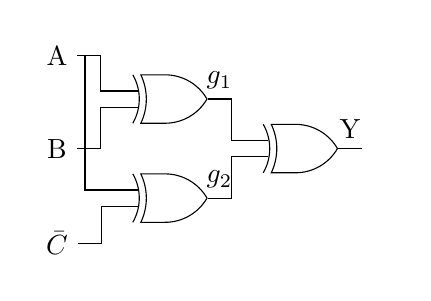
\begin{tikzpicture}[circuit logic US]
    \matrix[column sep=7mm]
    {
      \node (A) {A}; &  &  & \\
      & \node [xor gate] (AxorB) {}; &  &\\
      \node (B) {B}; &  & \node [xor gate] (f) {}; \\
      & \node [xor gate] (BxorC) {}; &  & \\
      \node (C) {$\bC$}; &  & &\\
    };
    \draw (A.east) --++(right:3mm) |- (AxorB.input 1);
    \draw (B.east) --++(right:3mm) |- (AxorB.input 2);
    \draw (A.east) --++(right:1mm) |- (BxorC.input 1);
    \draw (C.east) --++(right:3mm) |- (BxorC.input 2);
    \draw (AxorB.output) to [edge label=$g_1$] ++(right:3mm) |- (f.input 1);
    \draw (BxorC.output) to [edge label=$g_2$] ++(right:3mm) |- (f.input 2);
    \draw (f.output) to [edge label=Y] ++(right:3mm) ;
  \end{tikzpicture} \\
  By algebraic manipulation, prove or disprove that $Y = \bB \bC + B C$ (10 marks).
\end{prob}

\begin{prob}
Use the following 5-variable K-map for F (A, B, C, D, E), and find
  a minimal SOP expression for F (15 marks)\\
\begin{minipage}{0.5\linewidth}
  \centering
  \begin{Karnaugh}{BC}{DE}
    \minterms{0,1,5,6,7,8,9,14}
  \end{Karnaugh}\\
  A=0
\end{minipage}%
\begin{minipage}{0.5\linewidth}
  \centering
  \begin{Karnaugh}{BC}{DE}
    \minterms{1,4,5,6,7,9,12,14}
  \end{Karnaugh}\\
  A=1
\end{minipage}
\end{prob}

\begin{prob}
  Use bubble-pushing and/or algebra to find an SOP expression
for Y in the circuit below. If you use bubble-pushing, draw an equivalent
  circuit beside the given circuit (5 marks).\\
  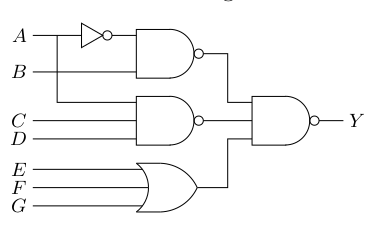
\includegraphics[width=0.4\linewidth]{figures/bubble-pushing-circuit.png}
\end{prob}

\begin{prob}
  Consider the function Y given below.
  \[ Y(A, B, C, D) = \sum m(0, 3, 5, 7, 8, 14) + d(2, 12, 15) \]
  \begin{enumerate}
    \item Draw a K-maps to derive a minimum SOP and POS expressions for Y .
      Indicate all essential prime implicants for Y or $\bY$ in your K-maps (20 marks).
    \item Sketch a two-level NOR-NOR circuit for Y. Assume that A, B, C, and D are available in true end complimentary forms (5 marks).
    \item Write Y in Product of sums (POS) \emph{canonical} form (5 marks).
  \end{enumerate}
\end{prob}

\begin{prob}
  Design a minimal SOP circuit to add two two-bit unsigned numbers. Denote the two bits of first number as $A_1A_0$ and the two bits of second number as $B_1B_0$. The result will be a 2-bit sum $S_1S_0$ and a carry $C$. Start with filling out the following truth table (3 example rows are provided) and then use K-maps to find minimal SOP for $S_1$, $S_0$ and a single carry bit $C_1$ (20 marks).
  \begin{tabular}{cccc|ccc}
    \toprule
    $A_1$ & $A_0$ & $B_1$ & $B_0$ & $C_1$ & $S_1$ & $S_0$  \\
    \midrule
    0 & 0 & 0 & 0 &   &   &   \\
    0 & 0 & 0 & 1 &   &   &   \\
    0 & 0 & 1 & 0 &   &   &   \\
    0 & 0 & 1 & 1 &   &   &   \\
    0 & 1 & 0 & 0 &   &   &   \\
    0 & 1 & 0 & 1 & 0 & 1 & 0 \\
    0 & 1 & 1 & 0 &   &   &   \\
    0 & 1 & 1 & 1 &   &   &   \\
    1 & 0 & 0 & 0 &   &   &   \\
    1 & 0 & 0 & 1 &   &   &   \\
    1 & 0 & 1 & 0 &   &   &   \\
    1 & 0 & 1 & 1 &   &   &   \\
    1 & 1 & 0 & 0 &   &   &   \\
    1 & 1 & 0 & 1 & 1 & 0 & 0 \\
    1 & 1 & 1 & 0 &   &   &   \\
    1 & 1 & 1 & 1 & 1 & 1 & 0 \\
    \bottomrule
  \end{tabular}
\end{prob}


%\bibliography{main}
%\bibliographystyle{plain}
\end{document}
